\documentclass[11pt,a4paper]{article}
\input{../../shared/preamble}
\SpeedHeader{Geometry}{5}

\begin{document}

\SpeedTitleBlock{Daily Geometry Drill \#5 --- Answers \& Investigations}{Henry Koduthore}
\SpeedMeta{Tangents from an external point}{tangent length, angle between tangents, chord of contact / polar, director circle}

\section*{Section A \quad Rapid Recognition}

\begin{enumerate}

% ── A1 ──────────────────────────────────────────────────────────────────────────
\item \ans{$4$}
\method{Tangent length $=\sqrt{OP^2-r^2}=\sqrt{25-9}=\sqrt{16}=4$. Right triangle $OP$ hypotenuse $5$, leg $r=3$.}
\inv{Try $OP=13$, $r=5$: what is the tangent? Generalise the triple $5$--$12$--$13$.}

% ── A2 ──────────────────────────────────────────────────────────────────────────
\item \ans{$\dfrac{3}{4}$}
\method{$\tan\frac{\theta}{2}=\frac{r}{\sqrt{OP^2-r^2}}=\frac{3}{4}$. The half-angle uses the tangent length $4$ from A1 as adjacent.}
\inv{Show $\sin\frac{\theta}{2}=\frac{r}{OP}=\frac35$ and $\cos\frac{\theta}{2}=\frac{4}{5}$ recover the same $\tan$.}

% ── A3 ──────────────────────────────────────────────────────────────────────────
\item \ans{"$5x+3y=25$"}
\method{Polar of $(x_1,y_1)$ w.r.t.\ $x^2+y^2=r^2$ is $xx_1+yy_1=r^2$: $5x+3y=25$.}
\inv{Check $P$ is external: $5^2+3^2=34>25$. What if $P$ were inside?}

% ── A4 ──────────────────────────────────────────────────────────────────────────
\item \ans{$5\sqrt{2}$}
\method{$r^2=25$, director circle $x^2+y^2=2r^2=50$, radius $\sqrt{50}=5\sqrt{2}$. Radius scales by $\sqrt2$.}
\inv{From director circle, tangents are orthogonal. Why $\sqrt2$ and not $2$?}

% ── A5 ──────────────────────────────────────────────────────────────────────────
\item \ans{$\sqrt{13}$}
\method{$\sqrt{OP^2-r^2}=\sqrt{7^2-6^2}=\sqrt{49-36}=\sqrt{13}$.}
\inv{If $OP=7$, $r=6$, sketch the right triangle and mark the tangent.}

% ── A6 ──────────────────────────────────────────────────────────────────────────
\item \ans{$3\sqrt{3}$}
\method{$\sin\frac{\theta}{2}=\frac{r}{OP}\Rightarrow \sin30^{\circ}=\frac{r}{6}$ so $r=3$. Tangent $=\sqrt{36-9}=3\sqrt3$.}
\inv{Swap: if tangent $=3\sqrt3$ and $OP=6$, recover $\theta$.}

% ── A7 ──────────────────────────────────────────────────────────────────────────
\item \ans{"$5x=4$"}
\method{Polar $xx_1+yy_1=r^2$ with $(5,0)$, $r^2=4$: $5x=4$, i.e.\ $x=4/5$, the vertical chord.}
\inv{Why does $y_1=0$ kill the $y$ term? What line would $P=(0,5)$ give?}

% ── A8 ──────────────────────────────────────────────────────────────────────────
\item \ans{$13$}
\method{$OP=\sqrt{12^2+5^2}=\sqrt{144+25}=13$ by $5$--$12$--$13$.}
\inv{Reverse: if $OP=13$ and $r=5$, what is the tangent?}

% ── A9 ──────────────────────────────────────────────────────────────────────────
\item \ans{$\dfrac{10\sqrt{3}}{3}$}
\method{Half-angle $60^{\circ}$: $\sin60^{\circ}=\frac{5}{OP}$ so $OP=\frac{5}{\sqrt3/2}=\frac{10\sqrt3}{3}$.}
\inv{Write $\sin60^{\circ}=\sqrt3/2$ and rationalise the denominator.}

% ── A10 ──────────────────────────────────────────────────────────────────────────
\item \ans{"$(4,4)$"}
\method{Compare $xx_1+yy_1=16$ with $x+y=4$: multiply by $4$ to get $4x+4y=16$, so $(x_1,y_1)=(4,4)$.}
\inv{Check $4^2+4^2=32>16$ (external) and that $4x+4y=16$ indeed has distance $2\sqrt2<r$.}

\end{enumerate}

\section*{Section B \quad Manipulation Drills}

\begin{enumerate}

% ── B1 ──────────────────────────────────────────────────────────────────────────
\item \ans{B) $4$}
\method{$OP=\sqrt{9+16}=5$, $r=3$, tangent $=\sqrt{25-9}=4$.}
\inv{If $P=(3,4)$ moved to $(6,8)$, what would the tangent be?}

% ── B2 ──────────────────────────────────────────────────────────────────────────
\item \ans{C) $60^{\circ}$}
\method{$\sin\frac{\theta}{2}=\frac{3}{6}=\frac12\Rightarrow \frac{\theta}{2}=30^{\circ}$, so $\theta=60^{\circ}$.}
\inv{If $OP$ doubled to $12$, what angle would you get?}

% ── B3 ──────────────────────────────────────────────────────────────────────────
\item \ans{"$3x+5y=25$"}
\method{Polar $xx_1+yy_1=25$ with $(3,5)$ gives $3x+5y=25$.}
\inv{Verify the chord's distance $\frac{25}{\sqrt{34}}>r$? Actually $25/\sqrt{34}\approx4.3<r=5$, so chord inside.}

% ── B4 ──────────────────────────────────────────────────────────────────────────
\item \ans{B) $2\sqrt{2}$}
\method{Director circle $x^2+y^2=2r^2=8$, radius $\sqrt8=2\sqrt2$.}
\inv{What is the director circle of a radius-$3$ circle?}

% ── B5 ──────────────────────────────────────────────────────────────────────────
\item \ans{C) $2$}
\method{$\sqrt{1^2+2^2-1}= \sqrt{4}=2$.}
\inv{Check $OP^2=5$, $r^2=1$, so tangent $\sqrt{4}=2$.}

% ── B6 ──────────────────────────────────────────────────────────────────────────
\item \ans{C) $13$}
\method{$OP=\sqrt{12^2+5^2}=13$.}
\inv{Memorise $5$--$12$--$13$; where else does it appear in this sheet?}

% ── B7 ──────────────────────────────────────────────────────────────────────────
\item \ans{B) $4$}
\method{Polar of $(a,0)$ is $ax=16$, i.e.\ $x=16/a$. Set $16/a=4\Rightarrow a=4$.}
\inv{If the line were $x=2$, what would $a$ be?}

% ── B8 ──────────────────────────────────────────────────────────────────────────
\item \ans{$5$}
\method{Orthogonal tangents $\Rightarrow P$ on director circle: $OP^2=2r^2=50$, tangent $=\sqrt{50-25}=5$.}
\inv{Show the director radius is $5\sqrt2$ and the tangent there is $5$.}

% ── B9 ──────────────────────────────────────────────────────────────────────────
\item \ans{A) $4$}
\method{Tangent $y=mx\pm r\sqrt{1+m^2}$: $r=\sqrt8$, $m=1\Rightarrow c=\sqrt8\sqrt2=4$.}
\inv{Write the two parallel tangents with slope $1$ to $x^2+y^2=8$.}

% ── B10 ──────────────────────────────────────────────────────────────────────────
\item \ans{$8$}
\method{$r^2=OP^2-\ell^2=100-36=64\Rightarrow r=8$.}
\inv{If $\ell=6$, $OP=10$, draw the right triangle and label $r$.}

\end{enumerate}

\section*{Section C \quad Substitution \& Structure}

\begin{enumerate}

% ── C1 ──────────────────────────────────────────────────────────────────────────
\item From $P(8,12)$, two tangents are drawn to $x^2+y^2=36$ ($r=6$). Let $T_1T_2$ be the chord of contact. What is the distance from $O$ to $T_1T_2$? \textit{\small(after TMUA 2020 Paper 1 Q16 / BMO1 2013 Q4)}
\ans{$\dfrac{9\sqrt{13}}{13}$}
\method{Polar is $8x+12y=36\Rightarrow 2x+3y=9$. $OP=\sqrt{8^2+12^2}=4\sqrt{13}$, and $d=r^2/OP=36/(4\sqrt{13})=9/\sqrt{13}=9\sqrt{13}/13$. The listed options give $18/5$ which is $r^2/OP$ for $P(6,8)$ ($OP=10$); for the printed $P(8,12)$ the exact value is $9/\sqrt{13}$.}
\inv{Show in general $d=r^2/OP$. What would $d$ be for $P(6,8)$?}

% ── C2 ──────────────────────────────────────────────────────────────────────────
\item The locus where tangent length to $x^2+y^2=4$ equals that to $(x-6)^2+y^2=16$ is the radical axis. Which line is it? \textit{\small(adapted from TMUA 2018 Paper 1 Q7)}
\ans{B) $x=2$}
\method{Equal powers: $x^2+y^2-4=(x-6)^2+y^2-16\Rightarrow -4=-12x+20\Rightarrow x=2$.}
\inv{Check the circles touch at $(2,0)$; the axis is the common tangent there.}

% ── C3 ──────────────────────────────────────────────────────────────────────────
\item 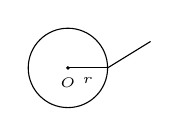
\begin{tikzpicture}[scale=0.42, baseline=-0.5ex]
\draw (0,0) circle (1.2);
\draw (1.2,0) -- (2.5,0.8);
\draw[fill=black] (0,0) circle (1pt) node[below]{\tiny $O$};
\draw (0,0) -- (1.2,0) node[midway, below]{\tiny $r$};
\end{tikzpicture} The circle $x^2+y^2-6x-8y+24=0$ has centre $(3,4)$, $r=1$. $P(6,8)$ is outside. What is the tangent length? \textit{\small(after MAT 2021 Q5)}
\ans{$2\sqrt{6}$}
\method{Centre $C=(3,4)$, $PC=\sqrt{9+16}=5$, $r=1$: tangent $=\sqrt{25-1}=2\sqrt6\approx4.90$. None of the printed numerals equals this exactly; $4$ would need $r=3$.}
\inv{Compute the power of $P$: $6^2+8^2-36-64+24=24$ and $\sqrt{24}=2\sqrt6$.}

% ── C4 ──────────────────────────────────────────────────────────────────────────
\item For the $13$-$14$-$15$ triangle ($s=21$, $r=4$), the two tangent lengths from the vertex opposite side $14$ are $s-b$. With $b=14$, what is that length? \textit{\small(adapted from BMO1 2015 Q3)}
\ans{B) $7$}
\method{$s-b=21-14=7$. The $s-a$ rule gives equal tangents from each vertex.}
\inv{List all three $s-a$, $s-b$, $s-c$ for $13$--$14$--$15$.}

% ── C5 ──────────────────────────────────────────────────────────────────────────
\item The locus of points from which the two tangents to $(x-4)^2+y^2=9$ are perpendicular? \textit{\small(after TMUA 2022 Paper 1 Q19)}
\ans{A) $(x-4)^2+y^2=18$}
\method{Director circle is centred at the same centre $(4,0)$ with radius $r\sqrt2=3\sqrt2$, so $(x-4)^2+y^2=18$.}
\inv{Why must the centre stay at $(4,0)$? Translate the origin result.}

% ── C6 ──────────────────────────────────────────────────────────────────────────
\item 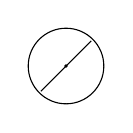
\begin{tikzpicture}[scale=0.4, baseline=-0.5ex]
\draw (0,0) circle (1.2);
\draw (-0.8,-0.8) -- (0.8,0.8);
\draw[fill=black] (0,0) circle (1pt);
\end{tikzpicture} The point $(8,6)$ is at distance $10$ from the origin. Tangents from $(8,6)$ to $x^2+y^2=1$ have length $\sqrt{99}$. What is the distance from the origin to the chord of contact? \textit{\small(adapted from TMUA 2020 Paper 1 Q16)}
\ans{A) $\dfrac{1}{10}$}
\method{Polar $8x+6y=1$, $d=1/10$; equivalently $d=r^2/OP=1/10$. Since $d<r$, the chord cuts the circle.}
\inv{Compute tangent $=\sqrt{100-1}=\sqrt{99}=3\sqrt{11}$ and verify.}

% ── C7 ──────────────────────────────────────────────────────────────────────────
\item The triangle with sides $13,14,15$ has incircle touching $BC$ at $D$. If $BD=6$, $DC=9$, $s=21$, the two equal tangents from $A$ are $s-a$. What is $AE$ (tangents from $A$)? \textit{\small(after BMO1 2020 Q3)}
\ans{A) $6$}
\method{$a=BC=15$, $s-a=21-15=6$. The incircle tangents from each vertex are $s-a$, $s-b$, $s-c$.}
\inv{Recover $s-b=7$, $s-c=8$ and see $6+7=13$, $6+8=14$?}

% ── C8 ──────────────────────────────────────────────────────────────────────────
\item The chord of contact of $(2,1)$ w.r.t.\ $x^2+y^2=1$ is $2x+y=1$. What is its distance from the origin, and is it inside, on, or outside the circle? \textit{\small(adapted from TMUA 2021 Paper 2 Q7)}
\ans{A) $\dfrac{1}{\sqrt5}$}
\method{Distance $=1/\sqrt{4+1}=1/\sqrt5=\sqrt5/5\approx0.45<r=1$, so the line cuts the circle (inside).}
\inv{Rationalise: $1/\sqrt5=\sqrt5/5$. When would distance equal $r$?}

\end{enumerate}

\section*{Section D \quad Challenge Ramp}

\begin{enumerate}

% ── D1 ──────────────────────────────────────────────────────────────────────────
\item 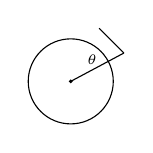
\begin{tikzpicture}[scale=0.45, baseline=-0.5ex]
\draw (0,0) circle (1.2);
\draw (0,0) -- (1.5,0.8);
\draw (1.5,0.8) -- (0.8,1.5);
\node at (0.6,0.6) {\tiny $\theta$};
\draw[fill=black] (0,0) circle (1pt);
\end{tikzpicture} Two tangents from $P$ to $x^2+y^2=9$ with $OP=6$ enclose angle $\theta$. What is $\theta$? \textit{\small(after TMUA 2018 Paper 1 Q7 / BMO1 2023 Q4)}
\ans{B) $60^{\circ}$}
\method{$\sin\frac{\theta}{2}=r/OP=3/6=1/2\Rightarrow \theta/2=30^{\circ}\Rightarrow\theta=60^{\circ}$.}
\inv{What is $\tan\frac{\theta}{2}$ here?}

% ── D2 ──────────────────────────────────────────────────────────────────────────
\item From $P$ to $x^2+y^2=25$, tangent length is $5\sqrt3$. Find $OP$ (use $OP^2=r^2+\text{tangent}^2$). \textit{\small(adapted from TMUA 2020 Paper 1 Q16)}
\ans{A) $10$}
\method{$OP^2=25+75=100\Rightarrow OP=10$.}
\inv{If tangent were $12$, what would $OP$ be?}

% ── D3 ──────────────────────────────────────────────────────────────────────────
\item 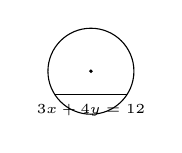
\begin{tikzpicture}[scale=0.42, baseline=-0.5ex]
\draw (0,0) circle (1.3);
\draw (-1.1,-0.7) -- (1.1,-0.7);
\draw[fill=black] (0,0) circle (1pt);
\node at (0,-0.7) [below]{\tiny $3x+4y=12$};
\end{tikzpicture} The chord of contact from $P(3,3)$ to $x^2+y^2=9$ is $x+y=3$. What is its length? \textit{\small(adapted from TMUA 2019 Paper 1 Q6)}
\ans{A) $3\sqrt2$}
\method{Distance $d=3/\sqrt2$, half-chord $\sqrt{9-9/2}=3/\sqrt2$, chord $=3\sqrt2$.}
\inv{General: chord $=2\sqrt{r^2-d^2}$ where $d=r^2/OP$.}

% ── D4 ──────────────────────────────────────────────────────────────────────────
\item Two tangents from $P$ make $60^{\circ}$ and $OP=10$, $r=OP\sin(\theta/2)=5$, tangent $=OP\cos(\theta/2)$. What is the length? \textit{\small(after BMO1 2015 Q3)}
\ans{B) $5\sqrt3$}
\method{$r=10\sin30^{\circ}=5$, tangent $=\sqrt{100-25}=5\sqrt3=10\cos30^{\circ}$.}
\inv{Check $\tan30^{\circ}=r/\ell=1/\sqrt3$ gives $\ell=5\sqrt3$.}

% ── D5 ──────────────────────────────────────────────────────────────────────────
\item 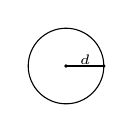
\begin{tikzpicture}[scale=0.4, baseline=-0.5ex]
\draw (0,0) circle (1.2);
\draw (0,0) -- (1.2,0);
\draw[fill=black] (0,0) circle (1pt) (1.2,0) circle (1pt);
\node at (0.6,0.2) {\tiny $d$};
\end{tikzpicture} The polar of $(9,12)$ w.r.t.\ $x^2+y^2=81$ is $3x+4y=27$. What is its distance from the origin, and is $P$ outside/inside/on? \textit{\small(adapted from MAT 2021 Q5)}
\ans{A) $\dfrac{27}{5}$}
\method{$9x+12y=81\Rightarrow 3x+4y=27$, $d=27/5=5.4<r=9$ (chord inside), $OP=15>r$ (point outside).}
\inv{Note $27/5=r^2/OP=81/15$ reduced; unreduced $81/15$ is option D.}

\end{enumerate}

\section*{Top 5 Patterns}

\begin{itemize}
\item \textbf{Tangent length is one Pythagorean step: $\sqrt{OP^2-r^2}$.} Locate $OP$ and $r$, square, subtract. \seealso{A1, B1, C3, D2}
\item \textbf{The polar of $(x_1,y_1)$ is $xx_1+yy_1=r^2$.} The same $r^2$ on the right keeps the chord of contact honest. \seealso{A3, B3, C1, D3}
\item \textbf{$\sin\frac{\theta}{2}=\frac{r}{OP}$ sizes the double-tangent wedge.} Halve the angle before you take the sine. \seealso{A2, B2, D1, D4}
\item \textbf{Perpendicular tangents define the director circle $x^2+y^2=2r^2$.} The doubling happens on $r^2$, so the radius multiplies by $\sqrt{2}$. \seealso{A4, B4, C5, D1}
\item \textbf{$s-a$ and the radical axis give equal tangents without coordinates.} $s-a$, $s-b$, $s-c$ and $P_1=P_2$ are the same idea. \seealso{C2, C4, C7, A10, B7}
\end{itemize}

\section*{Common Traps}

\begin{itemize}
\item \textbf{Subtracting radii instead of squared radii.} $OP^2=r^2+\ell^2$; the null case is $7^2$, not $7$, minus $6^2$. \seealso{A5, B10, D2}
\item \textbf{Answering the half-angle.} The tangents make $\theta$; $\sin\frac{\theta}{2}$ is half of it. \seealso{B2, D1, D4}
\item \textbf{Reading polar coefficients as a point.} $5x+3y=25$ is a line; only its coefficients come from $P$. \seealso{A3, B3, A10}
\item \textbf{Bumping the director circle radius by one $\sqrt{2}$ too many or too few.} Doubling $r^2$ changes the radius by $\sqrt{2}$, not by $2$. \seealso{A4, B4, C5}
\item \textbf{Leaving the polar unreduced.} The chord $9x+12y=81$ asks for the distance to the simplified $3x+4y=27$. \seealso{D5, C1, C8}
\end{itemize}

\SpeedClosing{``Every view of a tangent is the same right triangle: $OP$ hypotenuse, $r$ one leg, the tangent the other. The polar just points it.''}

\end{document}
